\begin{song}{title=\predtitle\centering Na co nesmíš zapomenout \\\large MIDI LIDI \vspace*{-0.3cm}}  %% sem se napíše jméno songu a autor
\moveright 1cm \vbox{      %Varianta č. 1  ---> Jeden sloupec zarovnaný na střed	
\begin{minipage}[t]{0.48\textwidth}\setlength{\parindent}{0.45cm}  %Varianta č. 2 --> Dva sloupce
\vetsi
\kapodastr{3}

\sloka
^{C}Tak jsem si přišel s tebou

^{F \z}popovídat, \\

a rady ti dát,

^{C}a rady ti dát.

\sloka
Na světe je dobře jenom

když ho máš rád,

ale kde to mám brát?

Ale kde to mám brát?

\sloka
Nemusíš už nikdy nechat

na sebe řvát,

tak do oka drát,

tak do oka drát.

\sloka
Že seš borec nemusíš už

na sebe hrát.

Trapný chvíle nejsou s tím,

kdo tě má rád.

\sloka
Nemusí ti překážet

prašivej stát,

můžeš občas taky něco

do rukou brát.

\sloka
Není nutný jenom doufat,

že to má řád,

můžeš ho ty tomu dát.

Můžeš ho ty tomu dát.

\end{minipage}\begin{minipage}[t]{0.48\textwidth}\setlength{\parindent}{0.45cm}\vspace*{0.55cm}  % V případě varianty č.2 jde odsud text do pravé části
\vetsi

[\textbf{Nejlepší mezihra}]

\sloka
^{C}A jestli už máš zas náladu

^{F \z}poraženou, \\

jestli si tvá hlava vzala

^{C \z}dovolenou. \\

A když se cítíš zas jak kafka

^{F \z}před proměnou,

tak ti zkusím ^{\z C\,\,}připomenout.

\sloka
A nemusíš se nikdy plazit

po kolenou.

Nenechej si prací zkazit

dovolenou.

A není nutný vždycky stát

na červenou,

ale vetšinou choď na zelenou.

\sloka
A nemusíš se vždycky jenom

holit pěnou.

Krize bývá rukou trhu

prodlouženou.

A jestli si chtěl večer strávit

se svou ženou,

tak na to nesmíš zapomenout!

\mezera

/: Tak na to nesmíš zapomenout. :/

\end{minipage}
}

\centering
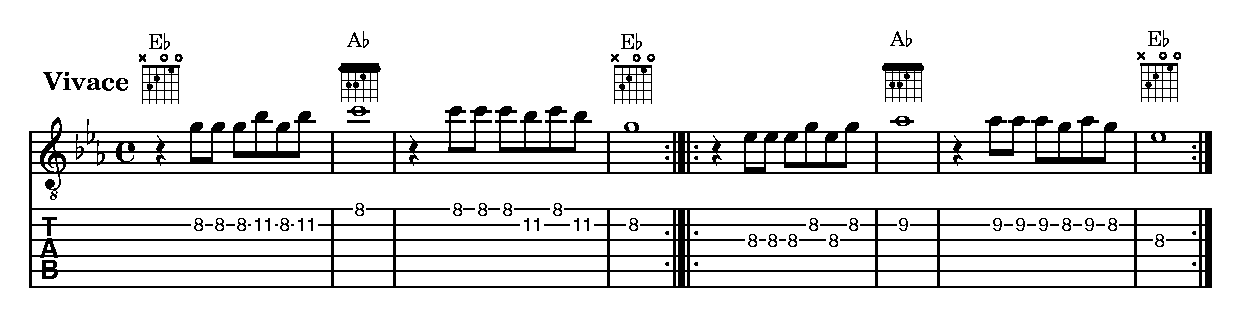
\includegraphics[scale=\defaulttabscale]{../taby/naconesmiszapomenout.pdf}

\setcounter{Slokočet}{0}
\end{song}
